\documentclass[1p]{elsarticle_modified}
%\bibliographystyle{elsarticle-num}

%\usepackage[colorlinks]{hyperref}
%\usepackage{abbrmath_seonhwa} %\Abb, \Ascr, \Acal ,\Abf, \Afrak
\usepackage{amsfonts}
\usepackage{amssymb}
\usepackage{amsmath}
\usepackage{amsthm}
\usepackage{scalefnt}
\usepackage{amsbsy}
\usepackage{kotex}
\usepackage{caption}
\usepackage{subfig}
\usepackage{color}
\usepackage{graphicx}
\usepackage{xcolor} %% white, black, red, green, blue, cyan, magenta, yellow
\usepackage{float}
\usepackage{setspace}
\usepackage{hyperref}

\usepackage{tikz}
\usetikzlibrary{arrows}

\usepackage{multirow}
\usepackage{array} % fixed length table
\usepackage{hhline}

%%%%%%%%%%%%%%%%%%%%%
\makeatletter
\renewcommand*\env@matrix[1][\arraystretch]{%
	\edef\arraystretch{#1}%
	\hskip -\arraycolsep
	\let\@ifnextchar\new@ifnextchar
	\array{*\c@MaxMatrixCols c}}
\makeatother %https://tex.stackexchange.com/questions/14071/how-can-i-increase-the-line-spacing-in-a-matrix
%%%%%%%%%%%%%%%

\usepackage[normalem]{ulem}

\newcommand{\msout}[1]{\ifmmode\text{\sout{\ensuremath{#1}}}\else\sout{#1}\fi}
%SOURCE: \msout is \stkout macro in https://tex.stackexchange.com/questions/20609/strikeout-in-math-mode

\newcommand{\cancel}[1]{
	\ifmmode
	{\color{red}\msout{#1}}
	\else
	{\color{red}\sout{#1}}
	\fi
}

\newcommand{\add}[1]{
	{\color{blue}\uwave{#1}}
}

\newcommand{\replace}[2]{
	\ifmmode
	{\color{red}\msout{#1}}{\color{blue}\uwave{#2}}
	\else
	{\color{red}\sout{#1}}{\color{blue}\uwave{#2}}
	\fi
}

\newcommand{\Sol}{\mathcal{S}} %segment
\newcommand{\D}{D} %diagram
\newcommand{\A}{\mathcal{A}} %arc


%%%%%%%%%%%%%%%%%%%%%%%%%%%%%5 test

\def\sl{\operatorname{\textup{SL}}(2,\Cbb)}
\def\psl{\operatorname{\textup{PSL}}(2,\Cbb)}
\def\quan{\mkern 1mu \triangleright \mkern 1mu}

\theoremstyle{definition}
\newtheorem{thm}{Theorem}[section]
\newtheorem{prop}[thm]{Proposition}
\newtheorem{lem}[thm]{Lemma}
\newtheorem{ques}[thm]{Question}
\newtheorem{cor}[thm]{Corollary}
\newtheorem{defn}[thm]{Definition}
\newtheorem{exam}[thm]{Example}
\newtheorem{rmk}[thm]{Remark}
\newtheorem{alg}[thm]{Algorithm}

\newcommand{\I}{\sqrt{-1}}
\begin{document}

%\begin{frontmatter}
%
%\title{Boundary parabolic representations of knots up to 8 crossings}
%
%%% Group authors per affiliation:
%\author{Yunhi Cho} 
%\address{Department of Mathematics, University of Seoul, Seoul, Korea}
%\ead{yhcho@uos.ac.kr}
%
%
%\author{Seonhwa Kim} %\fnref{s_kim}}
%\address{Center for Geometry and Physics, Institute for Basic Science, Pohang, 37673, Korea}
%\ead{ryeona17@ibs.re.kr}
%
%\author{Hyuk Kim}
%\address{Department of Mathematical Sciences, Seoul National University, Seoul 08826, Korea}
%\ead{hyukkim@snu.ac.kr}
%
%\author{Seokbeom Yoon}
%\address{Department of Mathematical Sciences, Seoul National University, Seoul, 08826,  Korea}
%\ead{sbyoon15@snu.ac.kr}
%
%\begin{abstract}
%We find all boundary parabolic representation of knots up to 8 crossings.
%
%\end{abstract}
%\begin{keyword}
%    \MSC[2010] 57M25 
%\end{keyword}
%
%\end{frontmatter}

%\linenumbers
%\tableofcontents
%
\newcommand\colored[1]{\textcolor{white}{\rule[-0.35ex]{0.8em}{1.4ex}}\kern-0.8em\color{red} #1}%
%\newcommand\colored[1]{\textcolor{white}{ #1}\kern-2.17ex	\textcolor{white}{ #1}\kern-1.81ex	\textcolor{white}{ #1}\kern-2.15ex\color{red}#1	}

{\Large $\underline{12a_{0304}~(K12a_{0304})}$}

\setlength{\tabcolsep}{10pt}
\renewcommand{\arraystretch}{1.6}
\vspace{1cm}\begin{tabular}{m{100pt}>{\centering\arraybackslash}m{274pt}}
\multirow{5}{120pt}{
	\centering
	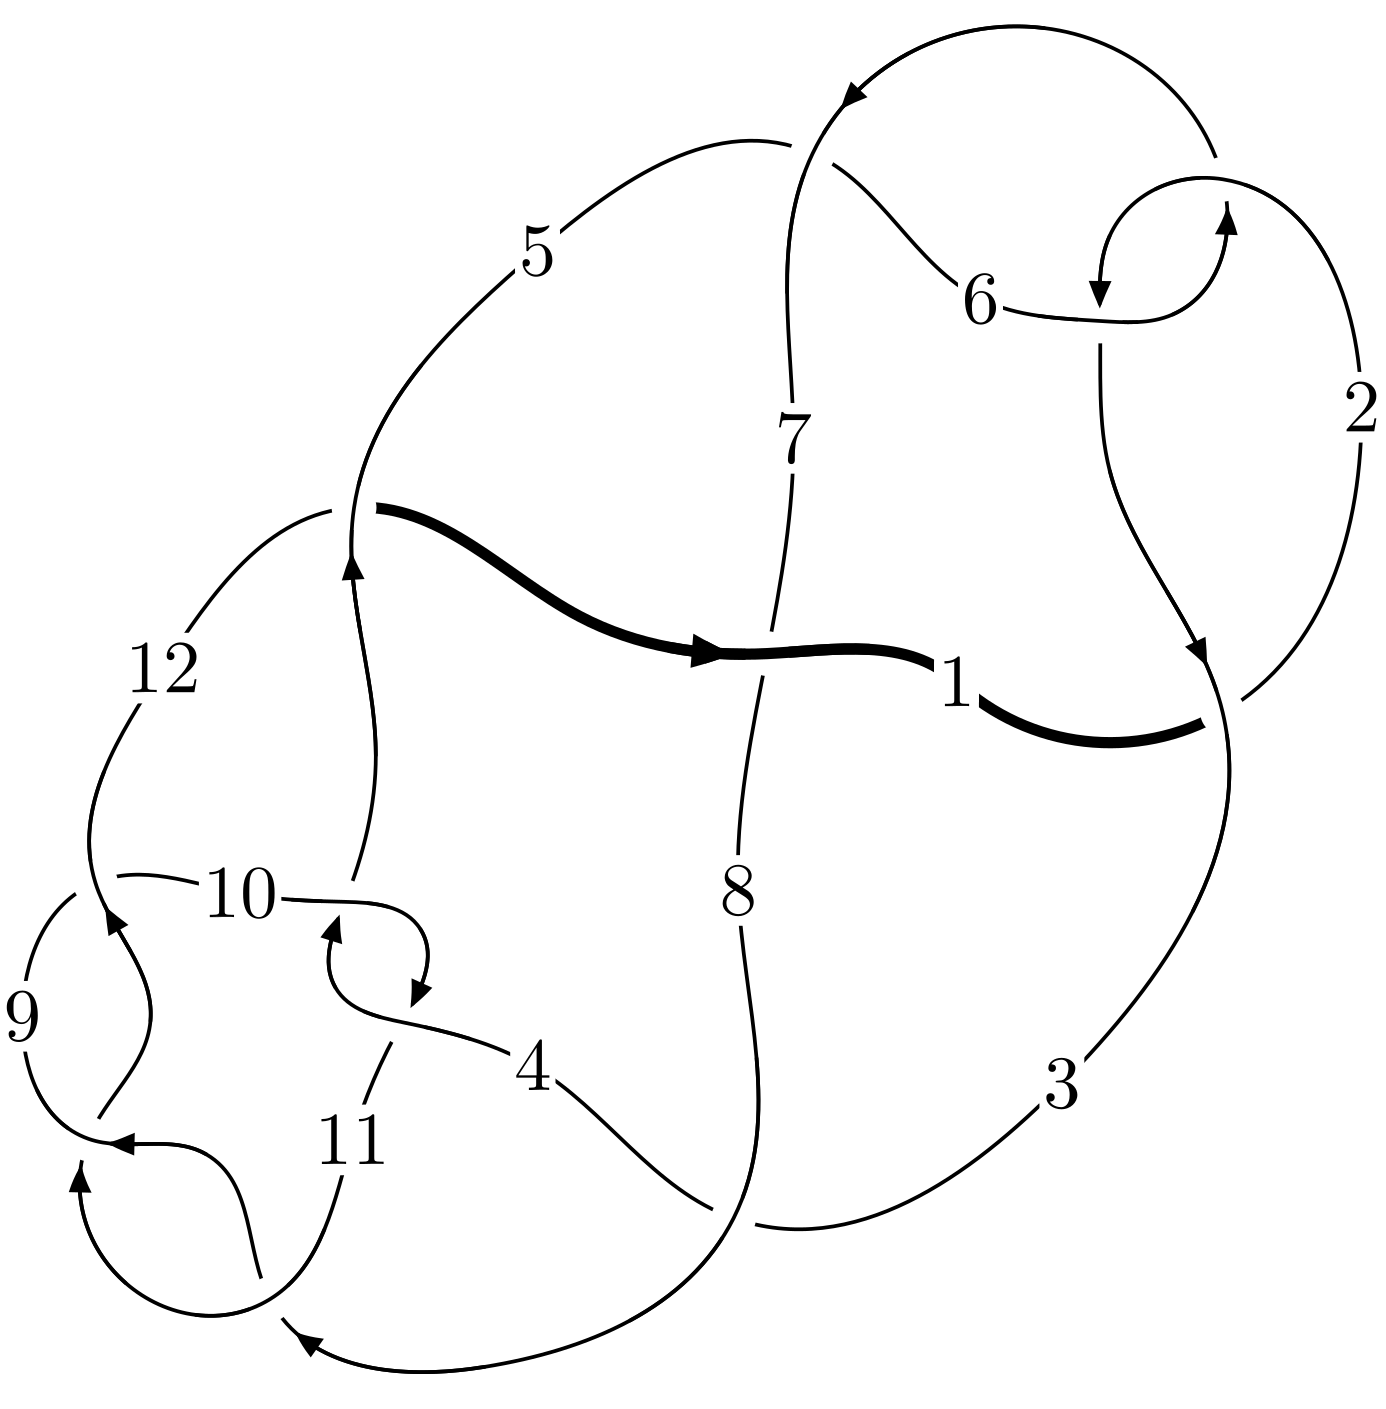
\includegraphics[width=112pt]{../../../GIT/diagram.site/Diagrams/png/1105_12a_0304.png}\\
\ \ \ A knot diagram\footnotemark}&
\allowdisplaybreaks
\textbf{Linearized knot diagam} \\
\cline{2-2}
 &
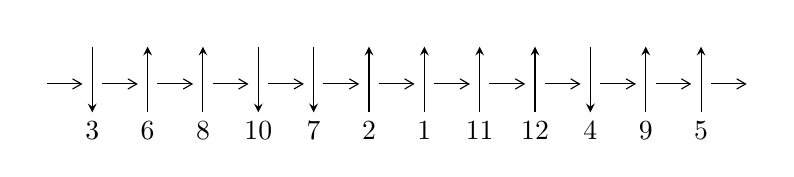
\begin{tikzpicture}[x=20pt, y=17pt]
	% nodes
	\node (C0) at (0, 0) {};
	\node (C1) at (1, 0) {};
	\node (C1U) at (1, +1) {};
	\node (C1D) at (1, -1) {3};

	\node (C2) at (2, 0) {};
	\node (C2U) at (2, +1) {};
	\node (C2D) at (2, -1) {6};

	\node (C3) at (3, 0) {};
	\node (C3U) at (3, +1) {};
	\node (C3D) at (3, -1) {8};

	\node (C4) at (4, 0) {};
	\node (C4U) at (4, +1) {};
	\node (C4D) at (4, -1) {10};

	\node (C5) at (5, 0) {};
	\node (C5U) at (5, +1) {};
	\node (C5D) at (5, -1) {7};

	\node (C6) at (6, 0) {};
	\node (C6U) at (6, +1) {};
	\node (C6D) at (6, -1) {2};

	\node (C7) at (7, 0) {};
	\node (C7U) at (7, +1) {};
	\node (C7D) at (7, -1) {1};

	\node (C8) at (8, 0) {};
	\node (C8U) at (8, +1) {};
	\node (C8D) at (8, -1) {11};

	\node (C9) at (9, 0) {};
	\node (C9U) at (9, +1) {};
	\node (C9D) at (9, -1) {12};

	\node (C10) at (10, 0) {};
	\node (C10U) at (10, +1) {};
	\node (C10D) at (10, -1) {4};

	\node (C11) at (11, 0) {};
	\node (C11U) at (11, +1) {};
	\node (C11D) at (11, -1) {9};

	\node (C12) at (12, 0) {};
	\node (C12U) at (12, +1) {};
	\node (C12D) at (12, -1) {5};
	\node (C13) at (13, 0) {};

	% arrows
	\draw[->,>={angle 60}]
	(C0) edge (C1) (C1) edge (C2) (C2) edge (C3) (C3) edge (C4) (C4) edge (C5) (C5) edge (C6) (C6) edge (C7) (C7) edge (C8) (C8) edge (C9) (C9) edge (C10) (C10) edge (C11) (C11) edge (C12) (C12) edge (C13) ;	\draw[->,>=stealth]
	(C1U) edge (C1D) (C2D) edge (C2U) (C3D) edge (C3U) (C4U) edge (C4D) (C5U) edge (C5D) (C6D) edge (C6U) (C7D) edge (C7U) (C8D) edge (C8U) (C9D) edge (C9U) (C10U) edge (C10D) (C11D) edge (C11U) (C12D) edge (C12U) ;
	\end{tikzpicture} \\
\hhline{~~} \\& 
\textbf{Solving Sequence} \\ \cline{2-2} 
 &
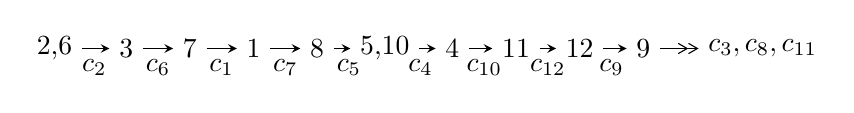
\begin{tikzpicture}[x=23pt, y=7pt]
	% node
	\node (A0) at (-1/8, 0) {2,6};
	\node (A1) at (1, 0) {3};
	\node (A2) at (2, 0) {7};
	\node (A3) at (3, 0) {1};
	\node (A4) at (4, 0) {8};
	\node (A5) at (81/16, 0) {5,10};
	\node (A6) at (49/8, 0) {4};
	\node (A7) at (57/8, 0) {11};
	\node (A8) at (65/8, 0) {12};
	\node (A9) at (73/8, 0) {9};
	\node (C1) at (1/2, -1) {$c_{2}$};
	\node (C2) at (3/2, -1) {$c_{6}$};
	\node (C3) at (5/2, -1) {$c_{1}$};
	\node (C4) at (7/2, -1) {$c_{7}$};
	\node (C5) at (9/2, -1) {$c_{5}$};
	\node (C6) at (45/8, -1) {$c_{4}$};
	\node (C7) at (53/8, -1) {$c_{10}$};
	\node (C8) at (61/8, -1) {$c_{12}$};
	\node (C9) at (69/8, -1) {$c_{9}$};
	\node (A10) at (11, 0) {$c_{3},c_{8},c_{11}$};

	% edge
	\draw[->,>=stealth]	
	(A0) edge (A1) (A1) edge (A2) (A2) edge (A3) (A3) edge (A4) (A4) edge (A5) (A5) edge (A6) (A6) edge (A7) (A7) edge (A8) (A8) edge (A9) ;
	\draw[->>,>={angle 60}]	
	(A9) edge (A10);
\end{tikzpicture} \\ 

\end{tabular} \\

\footnotetext{
The image of knot diagram is generated by the software ``\textbf{Draw programme}" developed by Andrew Bartholomew(\url{http://www.layer8.co.uk/maths/draw/index.htm\#Running-draw}), where we modified some parts for our purpose(\url{https://github.com/CATsTAILs/LinksPainter}).
}\phantom \\ \newline 
\centering \textbf{Ideals for irreducible components\footnotemark of $X_{\text{par}}$} 
 
\begin{align*}
I^u_{1}&=\langle 
2 u^{76}+u^{75}+\cdots+7 u^2+b,\;2 u^{76}+2 u^{75}+\cdots+a-1,\;u^{77}+2 u^{76}+\cdots- u-1\rangle \\
I^u_{2}&=\langle 
- u^8+u^7- u^6+u^5- u^4+u^3+b+u,\;u^6+u^4+u^2+a+u,\;u^9- u^8+2 u^7- u^6+3 u^5- u^4+2 u^3+u+1\rangle \\
\\
\end{align*}
\raggedright * 2 irreducible components of $\dim_{\mathbb{C}}=0$, with total 86 representations.\\
\footnotetext{All coefficients of polynomials are rational numbers. But the coefficients are sometimes approximated in decimal forms when there is not enough margin.}
\newpage
\renewcommand{\arraystretch}{1}
\centering \section*{I. $I^u_{1}= \langle 2 u^{76}+u^{75}+\cdots+7 u^2+b,\;2 u^{76}+2 u^{75}+\cdots+a-1,\;u^{77}+2 u^{76}+\cdots- u-1 \rangle$}
\flushleft \textbf{(i) Arc colorings}\\
\begin{tabular}{m{7pt} m{180pt} m{7pt} m{180pt} }
\flushright $a_{2}=$&$\begin{pmatrix}1\\0\end{pmatrix}$ \\
\flushright $a_{6}=$&$\begin{pmatrix}0\\u\end{pmatrix}$ \\
\flushright $a_{3}=$&$\begin{pmatrix}1\\- u^2\end{pmatrix}$ \\
\flushright $a_{7}=$&$\begin{pmatrix}u\\u\end{pmatrix}$ \\
\flushright $a_{1}=$&$\begin{pmatrix}u^2+1\\- u^4\end{pmatrix}$ \\
\flushright $a_{8}=$&$\begin{pmatrix}u^7+2 u^5+2 u^3+2 u\\- u^9- u^7- u^5+u\end{pmatrix}$ \\
\flushright $a_{5}=$&$\begin{pmatrix}u^3\\u^3+u\end{pmatrix}$ \\
\flushright $a_{10}=$&$\begin{pmatrix}-2 u^{76}-2 u^{75}+\cdots+5 u+1\\-2 u^{76}- u^{75}+\cdots-15 u^3-7 u^2\end{pmatrix}$ \\
\flushright $a_{4}=$&$\begin{pmatrix}- u^{14}-3 u^{12}-6 u^{10}-9 u^8-8 u^6-6 u^4-2 u^2+1\\u^{16}+2 u^{14}+4 u^{12}+4 u^{10}+2 u^8-2 u^4-2 u^2\end{pmatrix}$ \\
\flushright $a_{11}=$&$\begin{pmatrix}u^{73}+u^{72}+\cdots+8 u^2+5 u\\- u^{75}- u^{74}+\cdots-6 u^2- u\end{pmatrix}$ \\
\flushright $a_{12}=$&$\begin{pmatrix}u^{10}+u^8+2 u^6+u^4+u^2+1\\u^{10}+2 u^8+3 u^6+2 u^4+u^2\end{pmatrix}$ \\
\flushright $a_{9}=$&$\begin{pmatrix}- u^{76}- u^{75}+\cdots+6 u+1\\- u^{76}- u^{75}+\cdots-14 u^3-6 u^2\end{pmatrix}$\\&\end{tabular}
\flushleft \textbf{(ii) Obstruction class $= -1$}\\~\\
\flushleft \textbf{(iii) Cusp Shapes $= -4 u^{76}-6 u^{75}+\cdots+4 u+6$}\\~\\
\newpage\renewcommand{\arraystretch}{1}
\flushleft \textbf{(iv) u-Polynomials at the component}\newline \\
\begin{tabular}{m{50pt}|m{274pt}}
Crossings & \hspace{64pt}u-Polynomials at each crossing \\
\hline $$\begin{aligned}c_{1},c_{5}\end{aligned}$$&$\begin{aligned}
&u^{77}+24 u^{76}+\cdots+11 u-1
\end{aligned}$\\
\hline $$\begin{aligned}c_{2},c_{6}\end{aligned}$$&$\begin{aligned}
&u^{77}-2 u^{76}+\cdots- u+1
\end{aligned}$\\
\hline $$\begin{aligned}c_{3},c_{12}\end{aligned}$$&$\begin{aligned}
&u^{77}-2 u^{76}+\cdots-645 u+241
\end{aligned}$\\
\hline $$\begin{aligned}c_{4},c_{10}\end{aligned}$$&$\begin{aligned}
&u^{77}- u^{76}+\cdots+512 u+512
\end{aligned}$\\
\hline $$\begin{aligned}c_{7}\end{aligned}$$&$\begin{aligned}
&u^{77}+10 u^{76}+\cdots+45303 u+6643
\end{aligned}$\\
\hline $$\begin{aligned}c_{8},c_{9},c_{11}\end{aligned}$$&$\begin{aligned}
&u^{77}+10 u^{76}+\cdots+7 u+1
\end{aligned}$\\
\hline
\end{tabular}\\~\\
\newpage\renewcommand{\arraystretch}{1}
\flushleft \textbf{(v) Riley Polynomials at the component}\newline \\
\begin{tabular}{m{50pt}|m{274pt}}
Crossings & \hspace{64pt}Riley Polynomials at each crossing \\
\hline $$\begin{aligned}c_{1},c_{5}\end{aligned}$$&$\begin{aligned}
&y^{77}+60 y^{76}+\cdots+131 y-1
\end{aligned}$\\
\hline $$\begin{aligned}c_{2},c_{6}\end{aligned}$$&$\begin{aligned}
&y^{77}+24 y^{76}+\cdots+11 y-1
\end{aligned}$\\
\hline $$\begin{aligned}c_{3},c_{12}\end{aligned}$$&$\begin{aligned}
&y^{77}-72 y^{76}+\cdots-658353 y-58081
\end{aligned}$\\
\hline $$\begin{aligned}c_{4},c_{10}\end{aligned}$$&$\begin{aligned}
&y^{77}+57 y^{76}+\cdots+786432 y-262144
\end{aligned}$\\
\hline $$\begin{aligned}c_{7}\end{aligned}$$&$\begin{aligned}
&y^{77}-24 y^{76}+\cdots+567824027 y-44129449
\end{aligned}$\\
\hline $$\begin{aligned}c_{8},c_{9},c_{11}\end{aligned}$$&$\begin{aligned}
&y^{77}-80 y^{76}+\cdots+15 y-1
\end{aligned}$\\
\hline
\end{tabular}\\~\\
\newpage\flushleft \textbf{(vi) Complex Volumes and Cusp Shapes}
$$\begin{array}{c|c|c}  
\text{Solutions to }I^u_{1}& \I (\text{vol} + \sqrt{-1}CS) & \text{Cusp shape}\\
 \hline 
\begin{aligned}
u &= \phantom{-}0.699304 + 0.727429 I \\
a &= -0.81750 + 1.62981 I \\
b &= \phantom{-}1.09069 + 1.48911 I\end{aligned}
 & \phantom{-}1.98631 - 1.49498 I & \phantom{-0.000000 } 0 \\ \hline\begin{aligned}
u &= \phantom{-}0.699304 - 0.727429 I \\
a &= -0.81750 - 1.62981 I \\
b &= \phantom{-}1.09069 - 1.48911 I\end{aligned}
 & \phantom{-}1.98631 + 1.49498 I & \phantom{-0.000000 } 0 \\ \hline\begin{aligned}
u &= \phantom{-}0.744909 + 0.652303 I \\
a &= \phantom{-}1.26089 - 1.11132 I \\
b &= -0.58742 - 1.53965 I\end{aligned}
 & \phantom{-}7.63346 - 4.09071 I & \phantom{-}11.11372 + 0. I\phantom{ +0.000000I} \\ \hline\begin{aligned}
u &= \phantom{-}0.744909 - 0.652303 I \\
a &= \phantom{-}1.26089 + 1.11132 I \\
b &= -0.58742 + 1.53965 I\end{aligned}
 & \phantom{-}7.63346 + 4.09071 I & \phantom{-}11.11372 + 0. I\phantom{ +0.000000I} \\ \hline\begin{aligned}
u &= \phantom{-}0.255824 + 0.983693 I \\
a &= -2.12297 + 1.21195 I \\
b &= -0.696626 + 0.485271 I\end{aligned}
 & \phantom{-}2.47634 + 0.27430 I & \phantom{-0.000000 } 0 \\ \hline\begin{aligned}
u &= \phantom{-}0.255824 - 0.983693 I \\
a &= -2.12297 - 1.21195 I \\
b &= -0.696626 - 0.485271 I\end{aligned}
 & \phantom{-}2.47634 - 0.27430 I & \phantom{-0.000000 } 0 \\ \hline\begin{aligned}
u &= -0.170505 + 0.968417 I \\
a &= -0.123996 + 0.383932 I \\
b &= \phantom{-}0.236307 + 0.425064 I\end{aligned}
 & -1.37887 - 2.37996 I & \phantom{-0.000000 -}0. + 4.42703 I \\ \hline\begin{aligned}
u &= -0.170505 - 0.968417 I \\
a &= -0.123996 - 0.383932 I \\
b &= \phantom{-}0.236307 - 0.425064 I\end{aligned}
 & -1.37887 + 2.37996 I & \phantom{-0.000000 } 0. - 4.42703 I \\ \hline\begin{aligned}
u &= -0.049028 + 0.970113 I \\
a &= \phantom{-}0.677255 + 0.372469 I \\
b &= \phantom{-}0.574789 - 0.544320 I\end{aligned}
 & -3.09814 - 1.84421 I & -3.35735 + 5.07051 I \\ \hline\begin{aligned}
u &= -0.049028 - 0.970113 I \\
a &= \phantom{-}0.677255 - 0.372469 I \\
b &= \phantom{-}0.574789 + 0.544320 I\end{aligned}
 & -3.09814 + 1.84421 I & -3.35735 - 5.07051 I\\
 \hline 
 \end{array}$$\newpage$$\begin{array}{c|c|c}  
\text{Solutions to }I^u_{1}& \I (\text{vol} + \sqrt{-1}CS) & \text{Cusp shape}\\
 \hline 
\begin{aligned}
u &= -0.241315 + 1.005140 I \\
a &= \phantom{-}0.101331 - 0.745818 I \\
b &= -0.473125 - 0.927993 I\end{aligned}
 & \phantom{-}4.49560 - 2.98378 I & \phantom{-0.000000 } 0 \\ \hline\begin{aligned}
u &= -0.241315 - 1.005140 I \\
a &= \phantom{-}0.101331 + 0.745818 I \\
b &= -0.473125 + 0.927993 I\end{aligned}
 & \phantom{-}4.49560 + 2.98378 I & \phantom{-0.000000 } 0 \\ \hline\begin{aligned}
u &= -0.624221 + 0.829893 I \\
a &= \phantom{-}0.010477 + 0.678321 I \\
b &= -0.085050 + 0.648925 I\end{aligned}
 & \phantom{-}0.50764 - 1.96211 I & \phantom{-0.000000 } 0 \\ \hline\begin{aligned}
u &= -0.624221 - 0.829893 I \\
a &= \phantom{-}0.010477 - 0.678321 I \\
b &= -0.085050 - 0.648925 I\end{aligned}
 & \phantom{-}0.50764 + 1.96211 I & \phantom{-0.000000 } 0 \\ \hline\begin{aligned}
u &= \phantom{-}0.223875 + 1.016610 I \\
a &= \phantom{-}1.84493 - 1.38311 I \\
b &= \phantom{-}0.493359 - 0.072238 I\end{aligned}
 & \phantom{-}2.19034 + 5.64361 I & \phantom{-0.000000 } 0 \\ \hline\begin{aligned}
u &= \phantom{-}0.223875 - 1.016610 I \\
a &= \phantom{-}1.84493 + 1.38311 I \\
b &= \phantom{-}0.493359 + 0.072238 I\end{aligned}
 & \phantom{-}2.19034 - 5.64361 I & \phantom{-0.000000 } 0 \\ \hline\begin{aligned}
u &= -0.078493 + 1.040650 I \\
a &= -0.401232 - 0.523528 I \\
b &= -0.931882 + 0.327502 I\end{aligned}
 & \phantom{-}1.89327 - 3.83436 I & \phantom{-0.000000 } 0 \\ \hline\begin{aligned}
u &= -0.078493 - 1.040650 I \\
a &= -0.401232 + 0.523528 I \\
b &= -0.931882 - 0.327502 I\end{aligned}
 & \phantom{-}1.89327 + 3.83436 I & \phantom{-0.000000 } 0 \\ \hline\begin{aligned}
u &= \phantom{-}0.310575 + 0.996870 I \\
a &= \phantom{-}2.14157 - 1.01275 I \\
b &= \phantom{-}1.167780 - 0.616429 I\end{aligned}
 & \phantom{-}9.61828 - 3.45293 I & \phantom{-0.000000 } 0 \\ \hline\begin{aligned}
u &= \phantom{-}0.310575 - 0.996870 I \\
a &= \phantom{-}2.14157 + 1.01275 I \\
b &= \phantom{-}1.167780 + 0.616429 I\end{aligned}
 & \phantom{-}9.61828 + 3.45293 I & \phantom{-0.000000 } 0\\
 \hline 
 \end{array}$$\newpage$$\begin{array}{c|c|c}  
\text{Solutions to }I^u_{1}& \I (\text{vol} + \sqrt{-1}CS) & \text{Cusp shape}\\
 \hline 
\begin{aligned}
u &= -0.717183 + 0.773636 I \\
a &= -0.688793 - 1.001440 I \\
b &= -0.47922 - 1.34039 I\end{aligned}
 & \phantom{-}4.52846 - 0.10642 I & \phantom{-0.000000 } 0 \\ \hline\begin{aligned}
u &= -0.717183 - 0.773636 I \\
a &= -0.688793 + 1.001440 I \\
b &= -0.47922 + 1.34039 I\end{aligned}
 & \phantom{-}4.52846 + 0.10642 I & \phantom{-0.000000 } 0 \\ \hline\begin{aligned}
u &= \phantom{-}0.219337 + 1.048440 I \\
a &= -1.58099 + 1.23292 I \\
b &= -0.576448 - 0.293765 I\end{aligned}
 & \phantom{-}8.99981 + 9.75853 I & \phantom{-0.000000 } 0 \\ \hline\begin{aligned}
u &= \phantom{-}0.219337 - 1.048440 I \\
a &= -1.58099 - 1.23292 I \\
b &= -0.576448 + 0.293765 I\end{aligned}
 & \phantom{-}8.99981 - 9.75853 I & \phantom{-0.000000 } 0 \\ \hline\begin{aligned}
u &= \phantom{-}0.704904 + 0.820857 I \\
a &= -0.16649 - 2.37291 I \\
b &= -2.35033 - 1.28135 I\end{aligned}
 & \phantom{-}3.58538 + 2.22665 I & \phantom{-0.000000 } 0 \\ \hline\begin{aligned}
u &= \phantom{-}0.704904 - 0.820857 I \\
a &= -0.16649 + 2.37291 I \\
b &= -2.35033 + 1.28135 I\end{aligned}
 & \phantom{-}3.58538 - 2.22665 I & \phantom{-0.000000 } 0 \\ \hline\begin{aligned}
u &= \phantom{-}0.807197 + 0.737360 I \\
a &= -0.566438 - 0.328800 I \\
b &= -0.580161 + 0.466851 I\end{aligned}
 & \phantom{-}4.99997 - 1.53810 I & \phantom{-0.000000 } 0 \\ \hline\begin{aligned}
u &= \phantom{-}0.807197 - 0.737360 I \\
a &= -0.566438 + 0.328800 I \\
b &= -0.580161 - 0.466851 I\end{aligned}
 & \phantom{-}4.99997 + 1.53810 I & \phantom{-0.000000 } 0 \\ \hline\begin{aligned}
u &= \phantom{-}0.043394 + 0.902576 I \\
a &= -1.53012 - 0.31935 I \\
b &= -0.469965 + 0.858865 I\end{aligned}
 & -0.372258 + 0.930123 I & \phantom{-}1.97825 + 1.00417 I \\ \hline\begin{aligned}
u &= \phantom{-}0.043394 - 0.902576 I \\
a &= -1.53012 + 0.31935 I \\
b &= -0.469965 - 0.858865 I\end{aligned}
 & -0.372258 - 0.930123 I & \phantom{-}1.97825 - 1.00417 I\\
 \hline 
 \end{array}$$\newpage$$\begin{array}{c|c|c}  
\text{Solutions to }I^u_{1}& \I (\text{vol} + \sqrt{-1}CS) & \text{Cusp shape}\\
 \hline 
\begin{aligned}
u &= -0.563256 + 0.951321 I \\
a &= \phantom{-}0.866937 - 0.738751 I \\
b &= \phantom{-}1.091910 - 0.695769 I\end{aligned}
 & \phantom{-}4.66955 - 1.97768 I & \phantom{-0.000000 } 0 \\ \hline\begin{aligned}
u &= -0.563256 - 0.951321 I \\
a &= \phantom{-}0.866937 + 0.738751 I \\
b &= \phantom{-}1.091910 + 0.695769 I\end{aligned}
 & \phantom{-}4.66955 + 1.97768 I & \phantom{-0.000000 } 0 \\ \hline\begin{aligned}
u &= -0.837454 + 0.735539 I \\
a &= \phantom{-}0.97292 - 2.63486 I \\
b &= \phantom{-}3.85435 - 1.42730 I\end{aligned}
 & \phantom{-}9.14362 + 4.92278 I & \phantom{-0.000000 } 0 \\ \hline\begin{aligned}
u &= -0.837454 - 0.735539 I \\
a &= \phantom{-}0.97292 + 2.63486 I \\
b &= \phantom{-}3.85435 + 1.42730 I\end{aligned}
 & \phantom{-}9.14362 - 4.92278 I & \phantom{-0.000000 } 0 \\ \hline\begin{aligned}
u &= -0.848212 + 0.723641 I \\
a &= -0.65408 + 2.75056 I \\
b &= -3.60857 + 1.61834 I\end{aligned}
 & \phantom{-}16.0825 + 9.2947 I & \phantom{-0.000000 } 0 \\ \hline\begin{aligned}
u &= -0.848212 - 0.723641 I \\
a &= -0.65408 - 2.75056 I \\
b &= -3.60857 - 1.61834 I\end{aligned}
 & \phantom{-}16.0825 - 9.2947 I & \phantom{-0.000000 } 0 \\ \hline\begin{aligned}
u &= \phantom{-}0.837918 + 0.744240 I \\
a &= \phantom{-}1.131590 + 0.579415 I \\
b &= \phantom{-}1.08747 - 1.03259 I\end{aligned}
 & \phantom{-}11.50510 - 2.10024 I & \phantom{-0.000000 } 0 \\ \hline\begin{aligned}
u &= \phantom{-}0.837918 - 0.744240 I \\
a &= \phantom{-}1.131590 - 0.579415 I \\
b &= \phantom{-}1.08747 + 1.03259 I\end{aligned}
 & \phantom{-}11.50510 + 2.10024 I & \phantom{-0.000000 } 0 \\ \hline\begin{aligned}
u &= -0.646096 + 0.917216 I \\
a &= -0.846044 - 0.138690 I \\
b &= -0.772032 - 0.322959 I\end{aligned}
 & \phantom{-}0.20183 - 3.00562 I & \phantom{-0.000000 } 0 \\ \hline\begin{aligned}
u &= -0.646096 - 0.917216 I \\
a &= -0.846044 + 0.138690 I \\
b &= -0.772032 + 0.322959 I\end{aligned}
 & \phantom{-}0.20183 + 3.00562 I & \phantom{-0.000000 } 0\\
 \hline 
 \end{array}$$\newpage$$\begin{array}{c|c|c}  
\text{Solutions to }I^u_{1}& \I (\text{vol} + \sqrt{-1}CS) & \text{Cusp shape}\\
 \hline 
\begin{aligned}
u &= -0.833767 + 0.752545 I \\
a &= -1.13895 + 2.12752 I \\
b &= -3.71757 + 0.92447 I\end{aligned}
 & \phantom{-}9.45729 - 0.80584 I & \phantom{-0.000000 } 0 \\ \hline\begin{aligned}
u &= -0.833767 - 0.752545 I \\
a &= -1.13895 - 2.12752 I \\
b &= -3.71757 - 0.92447 I\end{aligned}
 & \phantom{-}9.45729 + 0.80584 I & \phantom{-0.000000 } 0 \\ \hline\begin{aligned}
u &= -0.842397 + 0.771277 I \\
a &= \phantom{-}0.72246 - 1.71278 I \\
b &= \phantom{-}3.13729 - 0.92017 I\end{aligned}
 & \phantom{-}16.9497 - 4.8229 I & \phantom{-0.000000 } 0 \\ \hline\begin{aligned}
u &= -0.842397 - 0.771277 I \\
a &= \phantom{-}0.72246 + 1.71278 I \\
b &= \phantom{-}3.13729 + 0.92017 I\end{aligned}
 & \phantom{-}16.9497 + 4.8229 I & \phantom{-0.000000 } 0 \\ \hline\begin{aligned}
u &= \phantom{-}0.695171 + 0.910303 I \\
a &= -1.68350 - 1.82196 I \\
b &= -3.07562 + 0.18717 I\end{aligned}
 & \phantom{-}3.30878 + 3.15042 I & \phantom{-0.000000 } 0 \\ \hline\begin{aligned}
u &= \phantom{-}0.695171 - 0.910303 I \\
a &= -1.68350 + 1.82196 I \\
b &= -3.07562 - 0.18717 I\end{aligned}
 & \phantom{-}3.30878 - 3.15042 I & \phantom{-0.000000 } 0 \\ \hline\begin{aligned}
u &= \phantom{-}0.778091 + 0.876907 I \\
a &= \phantom{-}0.78071 + 1.84733 I \\
b &= \phantom{-}2.58901 + 0.36941 I\end{aligned}
 & \phantom{-}11.68920 + 2.92576 I & \phantom{-0.000000 } 0 \\ \hline\begin{aligned}
u &= \phantom{-}0.778091 - 0.876907 I \\
a &= \phantom{-}0.78071 - 1.84733 I \\
b &= \phantom{-}2.58901 - 0.36941 I\end{aligned}
 & \phantom{-}11.68920 - 2.92576 I & \phantom{-0.000000 } 0 \\ \hline\begin{aligned}
u &= -0.701213 + 0.941339 I \\
a &= \phantom{-}1.24030 + 1.13056 I \\
b &= \phantom{-}0.57088 + 1.33782 I\end{aligned}
 & \phantom{-}4.01964 - 5.33236 I & \phantom{-0.000000 } 0 \\ \hline\begin{aligned}
u &= -0.701213 - 0.941339 I \\
a &= \phantom{-}1.24030 - 1.13056 I \\
b &= \phantom{-}0.57088 - 1.33782 I\end{aligned}
 & \phantom{-}4.01964 + 5.33236 I & \phantom{-0.000000 } 0\\
 \hline 
 \end{array}$$\newpage$$\begin{array}{c|c|c}  
\text{Solutions to }I^u_{1}& \I (\text{vol} + \sqrt{-1}CS) & \text{Cusp shape}\\
 \hline 
\begin{aligned}
u &= \phantom{-}0.686147 + 0.961876 I \\
a &= \phantom{-}1.75231 + 0.57908 I \\
b &= \phantom{-}2.14537 - 1.15325 I\end{aligned}
 & \phantom{-}1.28678 + 6.84249 I & \phantom{-0.000000 } 0 \\ \hline\begin{aligned}
u &= \phantom{-}0.686147 - 0.961876 I \\
a &= \phantom{-}1.75231 - 0.57908 I \\
b &= \phantom{-}2.14537 + 1.15325 I\end{aligned}
 & \phantom{-}1.28678 - 6.84249 I & \phantom{-0.000000 } 0 \\ \hline\begin{aligned}
u &= \phantom{-}0.685651 + 1.000130 I \\
a &= -1.67169 + 0.22266 I \\
b &= -1.46366 + 1.84464 I\end{aligned}
 & \phantom{-}6.61216 + 9.54266 I & \phantom{-0.000000 } 0 \\ \hline\begin{aligned}
u &= \phantom{-}0.685651 - 1.000130 I \\
a &= -1.67169 - 0.22266 I \\
b &= -1.46366 - 1.84464 I\end{aligned}
 & \phantom{-}6.61216 - 9.54266 I & \phantom{-0.000000 } 0 \\ \hline\begin{aligned}
u &= \phantom{-}0.736625 + 0.987761 I \\
a &= \phantom{-}0.098715 - 0.670264 I \\
b &= -0.640229 - 0.744065 I\end{aligned}
 & \phantom{-}4.23362 + 7.34344 I & \phantom{-0.000000 } 0 \\ \hline\begin{aligned}
u &= \phantom{-}0.736625 - 0.987761 I \\
a &= \phantom{-}0.098715 + 0.670264 I \\
b &= -0.640229 + 0.744065 I\end{aligned}
 & \phantom{-}4.23362 - 7.34344 I & \phantom{-0.000000 } 0 \\ \hline\begin{aligned}
u &= -0.757169 + 0.989788 I \\
a &= -2.14867 + 2.91335 I \\
b &= -3.80389 + 0.43415 I\end{aligned}
 & \phantom{-}8.72641 - 5.14321 I & \phantom{-0.000000 } 0 \\ \hline\begin{aligned}
u &= -0.757169 - 0.989788 I \\
a &= -2.14867 - 2.91335 I \\
b &= -3.80389 - 0.43415 I\end{aligned}
 & \phantom{-}8.72641 + 5.14321 I & \phantom{-0.000000 } 0 \\ \hline\begin{aligned}
u &= -0.771017 + 0.982703 I \\
a &= \phantom{-}1.78254 - 2.31369 I \\
b &= \phantom{-}3.04363 - 0.00238 I\end{aligned}
 & \phantom{-}16.2966 - 1.1968 I & \phantom{-0.000000 } 0 \\ \hline\begin{aligned}
u &= -0.771017 - 0.982703 I \\
a &= \phantom{-}1.78254 + 2.31369 I \\
b &= \phantom{-}3.04363 + 0.00238 I\end{aligned}
 & \phantom{-}16.2966 + 1.1968 I & \phantom{-0.000000 } 0\\
 \hline 
 \end{array}$$\newpage$$\begin{array}{c|c|c}  
\text{Solutions to }I^u_{1}& \I (\text{vol} + \sqrt{-1}CS) & \text{Cusp shape}\\
 \hline 
\begin{aligned}
u &= \phantom{-}0.755925 + 0.996210 I \\
a &= -0.272181 + 1.258230 I \\
b &= \phantom{-}1.18503 + 1.51805 I\end{aligned}
 & \phantom{-}10.72910 + 8.05684 I & \phantom{-0.000000 } 0 \\ \hline\begin{aligned}
u &= \phantom{-}0.755925 - 0.996210 I \\
a &= -0.272181 - 1.258230 I \\
b &= \phantom{-}1.18503 - 1.51805 I\end{aligned}
 & \phantom{-}10.72910 - 8.05684 I & \phantom{-0.000000 } 0 \\ \hline\begin{aligned}
u &= -0.751986 + 1.000640 I \\
a &= \phantom{-}2.80724 - 2.79451 I \\
b &= \phantom{-}4.40681 - 0.00361 I\end{aligned}
 & \phantom{-}8.32809 - 10.86460 I & \phantom{-0.000000 } 0 \\ \hline\begin{aligned}
u &= -0.751986 - 1.000640 I \\
a &= \phantom{-}2.80724 + 2.79451 I \\
b &= \phantom{-}4.40681 + 0.00361 I\end{aligned}
 & \phantom{-}8.32809 + 10.86460 I & \phantom{-0.000000 } 0 \\ \hline\begin{aligned}
u &= -0.752276 + 1.011150 I \\
a &= -2.96847 + 2.38538 I \\
b &= -4.43046 - 0.42786 I\end{aligned}
 & \phantom{-}15.1972 - 15.2671 I & \phantom{-0.000000 } 0 \\ \hline\begin{aligned}
u &= -0.752276 - 1.011150 I \\
a &= -2.96847 - 2.38538 I \\
b &= -4.43046 + 0.42786 I\end{aligned}
 & \phantom{-}15.1972 + 15.2671 I & \phantom{-0.000000 } 0 \\ \hline\begin{aligned}
u &= \phantom{-}0.689816 + 0.059020 I \\
a &= -0.29428 + 1.98529 I \\
b &= \phantom{-}0.338685 + 1.336490 I\end{aligned}
 & \phantom{-}12.6051 + 6.8095 I & \phantom{-}13.22063 - 3.73865 I \\ \hline\begin{aligned}
u &= \phantom{-}0.689816 - 0.059020 I \\
a &= -0.29428 - 1.98529 I \\
b &= \phantom{-}0.338685 - 1.336490 I\end{aligned}
 & \phantom{-}12.6051 - 6.8095 I & \phantom{-}13.22063 + 3.73865 I \\ \hline\begin{aligned}
u &= -0.663161\phantom{ +0.000000I} \\
a &= \phantom{-}1.42211\phantom{ +0.000000I} \\
b &= \phantom{-}0.101068\phantom{ +0.000000I}\end{aligned}
 & \phantom{-}7.71855\phantom{ +0.000000I} & \phantom{-}12.4530\phantom{ +0.000000I} \\ \hline\begin{aligned}
u &= -0.572725 + 0.325539 I \\
a &= \phantom{-}1.04804 - 1.33507 I \\
b &= \phantom{-}0.476521 - 0.202237 I\end{aligned}
 & \phantom{-}6.14632 - 2.18923 I & \phantom{-}11.48807 + 3.23279 I\\
 \hline 
 \end{array}$$\newpage$$\begin{array}{c|c|c}  
\text{Solutions to }I^u_{1}& \I (\text{vol} + \sqrt{-1}CS) & \text{Cusp shape}\\
 \hline 
\begin{aligned}
u &= -0.572725 - 0.325539 I \\
a &= \phantom{-}1.04804 + 1.33507 I \\
b &= \phantom{-}0.476521 + 0.202237 I\end{aligned}
 & \phantom{-}6.14632 + 2.18923 I & \phantom{-}11.48807 - 3.23279 I \\ \hline\begin{aligned}
u &= \phantom{-}0.658043 + 0.024681 I \\
a &= \phantom{-}0.12020 - 1.83501 I \\
b &= -0.17074 - 1.56090 I\end{aligned}
 & \phantom{-}5.53553 + 2.75768 I & \phantom{-}11.68630 - 3.17781 I \\ \hline\begin{aligned}
u &= \phantom{-}0.658043 - 0.024681 I \\
a &= \phantom{-}0.12020 + 1.83501 I \\
b &= -0.17074 + 1.56090 I\end{aligned}
 & \phantom{-}5.53553 - 2.75768 I & \phantom{-}11.68630 + 3.17781 I \\ \hline\begin{aligned}
u &= -0.561476\phantom{ +0.000000I} \\
a &= -0.758314\phantom{ +0.000000I} \\
b &= -0.0994541\phantom{ +0.000000I}\end{aligned}
 & \phantom{-}1.63385\phantom{ +0.000000I} & \phantom{-}5.54490\phantom{ +0.000000I} \\ \hline\begin{aligned}
u &= -0.295497 + 0.256148 I \\
a &= -0.84022 + 1.42123 I \\
b &= -0.128866 + 0.378321 I\end{aligned}
 & \phantom{-}0.365640 - 0.941295 I & \phantom{-}6.48634 + 7.23621 I \\ \hline\begin{aligned}
u &= -0.295497 - 0.256148 I \\
a &= -0.84022 - 1.42123 I \\
b &= -0.128866 - 0.378321 I\end{aligned}
 & \phantom{-}0.365640 + 0.941295 I & \phantom{-}6.48634 - 7.23621 I \\ \hline\begin{aligned}
u &= \phantom{-}0.266849\phantom{ +0.000000I} \\
a &= \phantom{-}1.64859\phantom{ +0.000000I} \\
b &= -0.897687\phantom{ +0.000000I}\end{aligned}
 & \phantom{-}2.07814\phantom{ +0.000000I} & \phantom{-}2.50950\phantom{ +0.000000I}\\
 \hline 
 \end{array}$$\newpage\newpage\renewcommand{\arraystretch}{1}
\centering \section*{II. $I^u_{2}= \langle - u^8+u^7- u^6+u^5- u^4+u^3+b+u,\;u^6+u^4+u^2+a+u,\;u^9- u^8+2 u^7- u^6+3 u^5- u^4+2 u^3+u+1 \rangle$}
\flushleft \textbf{(i) Arc colorings}\\
\begin{tabular}{m{7pt} m{180pt} m{7pt} m{180pt} }
\flushright $a_{2}=$&$\begin{pmatrix}1\\0\end{pmatrix}$ \\
\flushright $a_{6}=$&$\begin{pmatrix}0\\u\end{pmatrix}$ \\
\flushright $a_{3}=$&$\begin{pmatrix}1\\- u^2\end{pmatrix}$ \\
\flushright $a_{7}=$&$\begin{pmatrix}u\\u\end{pmatrix}$ \\
\flushright $a_{1}=$&$\begin{pmatrix}u^2+1\\- u^4\end{pmatrix}$ \\
\flushright $a_{8}=$&$\begin{pmatrix}u^7+2 u^5+2 u^3+2 u\\- u^8+u^7- u^6+2 u^5- u^4+2 u^3+2 u+1\end{pmatrix}$ \\
\flushright $a_{5}=$&$\begin{pmatrix}u^3\\u^3+u\end{pmatrix}$ \\
\flushright $a_{10}=$&$\begin{pmatrix}- u^6- u^4- u^2- u\\u^8- u^7+u^6- u^5+u^4- u^3- u\end{pmatrix}$ \\
\flushright $a_{4}=$&$\begin{pmatrix}u^3\\u^3+u\end{pmatrix}$ \\
\flushright $a_{11}=$&$\begin{pmatrix}- u^6- u^4- u^2- u\\u^8- u^7+u^6- u^5+u^4- u^3- u\end{pmatrix}$ \\
\flushright $a_{12}=$&$\begin{pmatrix}- u^7-2 u^5-2 u^3-2 u\\u^8- u^7+u^6-2 u^5+u^4-2 u^3-2 u-1\end{pmatrix}$ \\
\flushright $a_{9}=$&$\begin{pmatrix}u^7- u^6+2 u^5- u^4+2 u^3- u^2+u\\u^5+u^3+u+1\end{pmatrix}$\\&\end{tabular}
\flushleft \textbf{(ii) Obstruction class $= 1$}\\~\\
\flushleft \textbf{(iii) Cusp Shapes $= -4 u^7+4 u^6-5 u^5+5 u^4-10 u^3+5 u^2- u+11$}\\~\\
\newpage\renewcommand{\arraystretch}{1}
\flushleft \textbf{(iv) u-Polynomials at the component}\newline \\
\begin{tabular}{m{50pt}|m{274pt}}
Crossings & \hspace{64pt}u-Polynomials at each crossing \\
\hline $$\begin{aligned}c_{1},c_{5}\end{aligned}$$&$\begin{aligned}
&u^9-3 u^8+8 u^7-13 u^6+17 u^5-17 u^4+12 u^3-6 u^2+u+1
\end{aligned}$\\
\hline $$\begin{aligned}c_{2}\end{aligned}$$&$\begin{aligned}
&u^9- u^8+2 u^7- u^6+3 u^5- u^4+2 u^3+u+1
\end{aligned}$\\
\hline $$\begin{aligned}c_{3},c_{12}\end{aligned}$$&$\begin{aligned}
&u^9- u^8-2 u^7+3 u^6+u^5-3 u^4+2 u^3- u+1
\end{aligned}$\\
\hline $$\begin{aligned}c_{4},c_{10}\end{aligned}$$&$\begin{aligned}
&u^9
\end{aligned}$\\
\hline $$\begin{aligned}c_{6}\end{aligned}$$&$\begin{aligned}
&u^9+u^8+2 u^7+u^6+3 u^5+u^4+2 u^3+u-1
\end{aligned}$\\
\hline $$\begin{aligned}c_{7}\end{aligned}$$&$\begin{aligned}
&u^9-5 u^8+12 u^7-15 u^6+9 u^5+u^4-4 u^3+2 u^2+u-1
\end{aligned}$\\
\hline $$\begin{aligned}c_{8},c_{9}\end{aligned}$$&$\begin{aligned}
&(u+1)^9
\end{aligned}$\\
\hline $$\begin{aligned}c_{11}\end{aligned}$$&$\begin{aligned}
&(u-1)^9
\end{aligned}$\\
\hline
\end{tabular}\\~\\
\newpage\renewcommand{\arraystretch}{1}
\flushleft \textbf{(v) Riley Polynomials at the component}\newline \\
\begin{tabular}{m{50pt}|m{274pt}}
Crossings & \hspace{64pt}Riley Polynomials at each crossing \\
\hline $$\begin{aligned}c_{1},c_{5}\end{aligned}$$&$\begin{aligned}
&y^9+7 y^8+20 y^7+25 y^6+5 y^5-15 y^4+22 y^2+13 y-1
\end{aligned}$\\
\hline $$\begin{aligned}c_{2},c_{6}\end{aligned}$$&$\begin{aligned}
&y^9+3 y^8+8 y^7+13 y^6+17 y^5+17 y^4+12 y^3+6 y^2+y-1
\end{aligned}$\\
\hline $$\begin{aligned}c_{3},c_{12}\end{aligned}$$&$\begin{aligned}
&y^9-5 y^8+12 y^7-15 y^6+9 y^5+y^4-4 y^3+2 y^2+y-1
\end{aligned}$\\
\hline $$\begin{aligned}c_{4},c_{10}\end{aligned}$$&$\begin{aligned}
&y^9
\end{aligned}$\\
\hline $$\begin{aligned}c_{7}\end{aligned}$$&$\begin{aligned}
&y^9- y^8+12 y^7-7 y^6+37 y^5+y^4-10 y^2+5 y-1
\end{aligned}$\\
\hline $$\begin{aligned}c_{8},c_{9},c_{11}\end{aligned}$$&$\begin{aligned}
&(y-1)^9
\end{aligned}$\\
\hline
\end{tabular}\\~\\
\newpage\flushleft \textbf{(vi) Complex Volumes and Cusp Shapes}
$$\begin{array}{c|c|c}  
\text{Solutions to }I^u_{2}& \I (\text{vol} + \sqrt{-1}CS) & \text{Cusp shape}\\
 \hline 
\begin{aligned}
u &= -0.140343 + 0.966856 I \\
a &= \phantom{-}0.855828 - 0.530357 I \\
b &= \phantom{-}0.154190 + 0.257272 I\end{aligned}
 & -0.13850 - 2.09337 I & \phantom{-}4.27981 + 4.44592 I \\ \hline\begin{aligned}
u &= -0.140343 - 0.966856 I \\
a &= \phantom{-}0.855828 + 0.530357 I \\
b &= \phantom{-}0.154190 - 0.257272 I\end{aligned}
 & -0.13850 + 2.09337 I & \phantom{-}4.27981 - 4.44592 I \\ \hline\begin{aligned}
u &= -0.628449 + 0.875112 I \\
a &= \phantom{-}0.77654 - 1.46791 I \\
b &= \phantom{-}1.76111 - 0.42995 I\end{aligned}
 & \phantom{-}2.26187 - 2.45442 I & \phantom{-}4.16203 + 2.47153 I \\ \hline\begin{aligned}
u &= -0.628449 - 0.875112 I \\
a &= \phantom{-}0.77654 + 1.46791 I \\
b &= \phantom{-}1.76111 + 0.42995 I\end{aligned}
 & \phantom{-}2.26187 + 2.45442 I & \phantom{-}4.16203 - 2.47153 I \\ \hline\begin{aligned}
u &= \phantom{-}0.796005 + 0.733148 I \\
a &= \phantom{-}0.852888 - 0.566992 I \\
b &= \phantom{-}0.430151 - 1.332530 I\end{aligned}
 & \phantom{-}6.01628 - 1.33617 I & \phantom{-}13.03110 + 0.17445 I \\ \hline\begin{aligned}
u &= \phantom{-}0.796005 - 0.733148 I \\
a &= \phantom{-}0.852888 + 0.566992 I \\
b &= \phantom{-}0.430151 + 1.332530 I\end{aligned}
 & \phantom{-}6.01628 + 1.33617 I & \phantom{-}13.03110 - 0.17445 I \\ \hline\begin{aligned}
u &= \phantom{-}0.728966 + 0.986295 I \\
a &= -1.06667 + 0.97795 I \\
b &= -0.23704 + 1.46509 I\end{aligned}
 & \phantom{-}5.24306 + 7.08493 I & \phantom{-}11.12684 - 5.18429 I \\ \hline\begin{aligned}
u &= \phantom{-}0.728966 - 0.986295 I \\
a &= -1.06667 - 0.97795 I \\
b &= -0.23704 - 1.46509 I\end{aligned}
 & \phantom{-}5.24306 - 7.08493 I & \phantom{-}11.12684 + 5.18429 I \\ \hline\begin{aligned}
u &= -0.512358\phantom{ +0.000000I} \\
a &= \phantom{-}0.162845\phantom{ +0.000000I} \\
b &= \phantom{-}0.783184\phantom{ +0.000000I}\end{aligned}
 & \phantom{-}2.84338\phantom{ +0.000000I} & \phantom{-}14.8000\phantom{ +0.000000I}\\
 \hline 
 \end{array}$$\newpage
\newpage\renewcommand{\arraystretch}{1}
\centering \section*{ III. u-Polynomials}
\begin{tabular}{m{50pt}|m{274pt}}
Crossings & \hspace{64pt}u-Polynomials at each crossing \\
\hline $$\begin{aligned}c_{1},c_{5}\end{aligned}$$&$\begin{aligned}
&(u^9-3 u^8+8 u^7-13 u^6+17 u^5-17 u^4+12 u^3-6 u^2+u+1)\\
&\cdot(u^{77}+24 u^{76}+\cdots+11 u-1)
\end{aligned}$\\
\hline $$\begin{aligned}c_{2}\end{aligned}$$&$\begin{aligned}
&(u^9- u^8+\cdots+u+1)(u^{77}-2 u^{76}+\cdots- u+1)
\end{aligned}$\\
\hline $$\begin{aligned}c_{3},c_{12}\end{aligned}$$&$\begin{aligned}
&(u^9- u^8-2 u^7+3 u^6+u^5-3 u^4+2 u^3- u+1)\\
&\cdot(u^{77}-2 u^{76}+\cdots-645 u+241)
\end{aligned}$\\
\hline $$\begin{aligned}c_{4},c_{10}\end{aligned}$$&$\begin{aligned}
&u^9(u^{77}- u^{76}+\cdots+512 u+512)
\end{aligned}$\\
\hline $$\begin{aligned}c_{6}\end{aligned}$$&$\begin{aligned}
&(u^9+u^8+\cdots+u-1)(u^{77}-2 u^{76}+\cdots- u+1)
\end{aligned}$\\
\hline $$\begin{aligned}c_{7}\end{aligned}$$&$\begin{aligned}
&(u^9-5 u^8+12 u^7-15 u^6+9 u^5+u^4-4 u^3+2 u^2+u-1)\\
&\cdot(u^{77}+10 u^{76}+\cdots+45303 u+6643)
\end{aligned}$\\
\hline $$\begin{aligned}c_{8},c_{9}\end{aligned}$$&$\begin{aligned}
&((u+1)^9)(u^{77}+10 u^{76}+\cdots+7 u+1)
\end{aligned}$\\
\hline $$\begin{aligned}c_{11}\end{aligned}$$&$\begin{aligned}
&((u-1)^9)(u^{77}+10 u^{76}+\cdots+7 u+1)
\end{aligned}$\\
\hline
\end{tabular}\newpage\renewcommand{\arraystretch}{1}
\centering \section*{ IV. Riley Polynomials}
\begin{tabular}{m{50pt}|m{274pt}}
Crossings & \hspace{64pt}Riley Polynomials at each crossing \\
\hline $$\begin{aligned}c_{1},c_{5}\end{aligned}$$&$\begin{aligned}
&(y^9+7 y^8+20 y^7+25 y^6+5 y^5-15 y^4+22 y^2+13 y-1)\\
&\cdot(y^{77}+60 y^{76}+\cdots+131 y-1)
\end{aligned}$\\
\hline $$\begin{aligned}c_{2},c_{6}\end{aligned}$$&$\begin{aligned}
&(y^9+3 y^8+8 y^7+13 y^6+17 y^5+17 y^4+12 y^3+6 y^2+y-1)\\
&\cdot(y^{77}+24 y^{76}+\cdots+11 y-1)
\end{aligned}$\\
\hline $$\begin{aligned}c_{3},c_{12}\end{aligned}$$&$\begin{aligned}
&(y^9-5 y^8+12 y^7-15 y^6+9 y^5+y^4-4 y^3+2 y^2+y-1)\\
&\cdot(y^{77}-72 y^{76}+\cdots-658353 y-58081)
\end{aligned}$\\
\hline $$\begin{aligned}c_{4},c_{10}\end{aligned}$$&$\begin{aligned}
&y^9(y^{77}+57 y^{76}+\cdots+786432 y-262144)
\end{aligned}$\\
\hline $$\begin{aligned}c_{7}\end{aligned}$$&$\begin{aligned}
&(y^9- y^8+12 y^7-7 y^6+37 y^5+y^4-10 y^2+5 y-1)\\
&\cdot(y^{77}-24 y^{76}+\cdots+567824027 y-44129449)
\end{aligned}$\\
\hline $$\begin{aligned}c_{8},c_{9},c_{11}\end{aligned}$$&$\begin{aligned}
&((y-1)^9)(y^{77}-80 y^{76}+\cdots+15 y-1)
\end{aligned}$\\
\hline
\end{tabular}
\vskip 2pc
\end{document}